\documentclass[12pt]{article}

\usepackage[a4paper,width=160mm,top=20mm,bottom=20mm,bindingoffset=6mm]{geometry}
\usepackage{graphicx}
\usepackage{caption}
\usepackage{subcaption}

\title{Affordable drone education platform}

\date{September 10, 2016}

\author{
	Sundaramahalingam, Sudharshan\\
	\and
	Isaac Tay Eng Hian\\
	\and
	Ambrose Chua\\
	\and
	Prahlad Vadakkepat
}

\begin{document}

\maketitle
\pagenumbering{gobble}
\newpage
\pagenumbering{arabic}

\section{Introduction}

The Unmanned Aerial Vehicle (UAV), commonly known as a drone, industry has seen a market growth from a 552 million USD industry in 2014, to 1.4 billion USD in 2015 with an expected forecast of 5 billion USD by 2017.\cite{legalandsocial} Drones are being applied to practical uses in agriculture, surveillance, security and industrial automation. One application of drones is a military attack platform where the industry is estimated to reach 1.8 trillion by 2017.\cite{dronewars} Another application is in the agriculture industry through monitoring of crops, large plantations and vegetation.[3] Specialized applications include mosquito vector control[4] and oil spill detection monitoring[5]. 

Drones are increasingly being used as a platform for robotics research, secondary and higher education.[6] Drones are suitable to facilitate learning especially in robotics, control systems, embedded system engineering, artificial intelligence and systems engineering.[7] Additionally, they could be used to teach concepts like Bernoulli’s principle, stall speed, practical circuitry, fluid dynamics, and projectile motion to secondary education students.

Quadrotor helicopters or quadcopters are currently the most common drone platforms available. They operate on the mechanics of 4 rotors spinning at varying velocities which allows the drone to achieve steering and thrust through a PID loop based control system.[8] These quadcopters are unaffordable in large quantities for integration into schools. Quadrotor platforms also have exposed rotors which raises safety concerns for use in schools. Although these platforms have free APIs, the hardware is closed-source making it hard for students to explore and delve into hardware based topics using these platforms.

An affordable and open architecture drone, namely SentiBot, is detailed in this work. SentiBot utilizes a dual-propeller electronic ducted fan (EDF) with an enclosed frame in a coax-copter design. The design increases safety while decreasing the cost and enables high modularity. The frame is 3D-printed which allows easy hardware replication for experimentation to be conducted with additional sensors. The platform has the Intel Edison System on a Chip (SoC) and a unique dual CPU architecture which enables compartmentalization of computational tasks. 9] The higher level tasks are managed by the Intel Edison CPU while the lower level real-time tasks are handled by the ATMEGA 328 8-bit microcontroller running a real time operating system (RTOS). The platform utilizes Yocto Linux and supports ROS which provides open source libraries and software resources.[10]

\section{SentiBot hardware design}

\subsection{Safety, affordability and accessibility of educational platform}

The concern with drone safety has resulted in the stringent regulation by governments on the usage of drones in public and in industries.[11] The safety of the drone is thus critical. A lower cost drone platform allows a greater adoption rate by schools as budget cuts faced by schools is impacting adoption of a technology based curriculum.[12] Robotics platforms used in education need to provide easy access to hardware and software systems to enable students to learn through experimentation.[13] The three aspects of an education drone platform is summarized as safety, affordability and accessibility. 

\subsection{Modular, 3D printed drone frame design}

The Sentibot uses a novel frame design which is made through additive material fabrication using a Nylon-6 filament as Nylon-6 provides a high durability to weight ratio which is favorable for a flying platform.[14] The novelty of the design is that the electronics in housed outside of the main body in contrast to the internal housing seen in other coax copters.[15] Having the electronics outside the main body enhances the accessibility of the electronics components. 

A modular frame design based on support beams holds the frame together. The frame is designed in a cylindrical form as the compressive strength of cylinders has been shown to be superior of cuboids due to lack of discrete stress points like the corners of a cuboid[16] A two part motor assembly is used to enclose 2 counter-rotating rotors which creating a ducting effect. The ducting of the motors increases efficiency at high rotary speeds and also enhances the static thrust performance of the system.[17] 

\begin{figure}
	\centering
	\begin{subfigure}{0.5\textwidth}
		\centering
		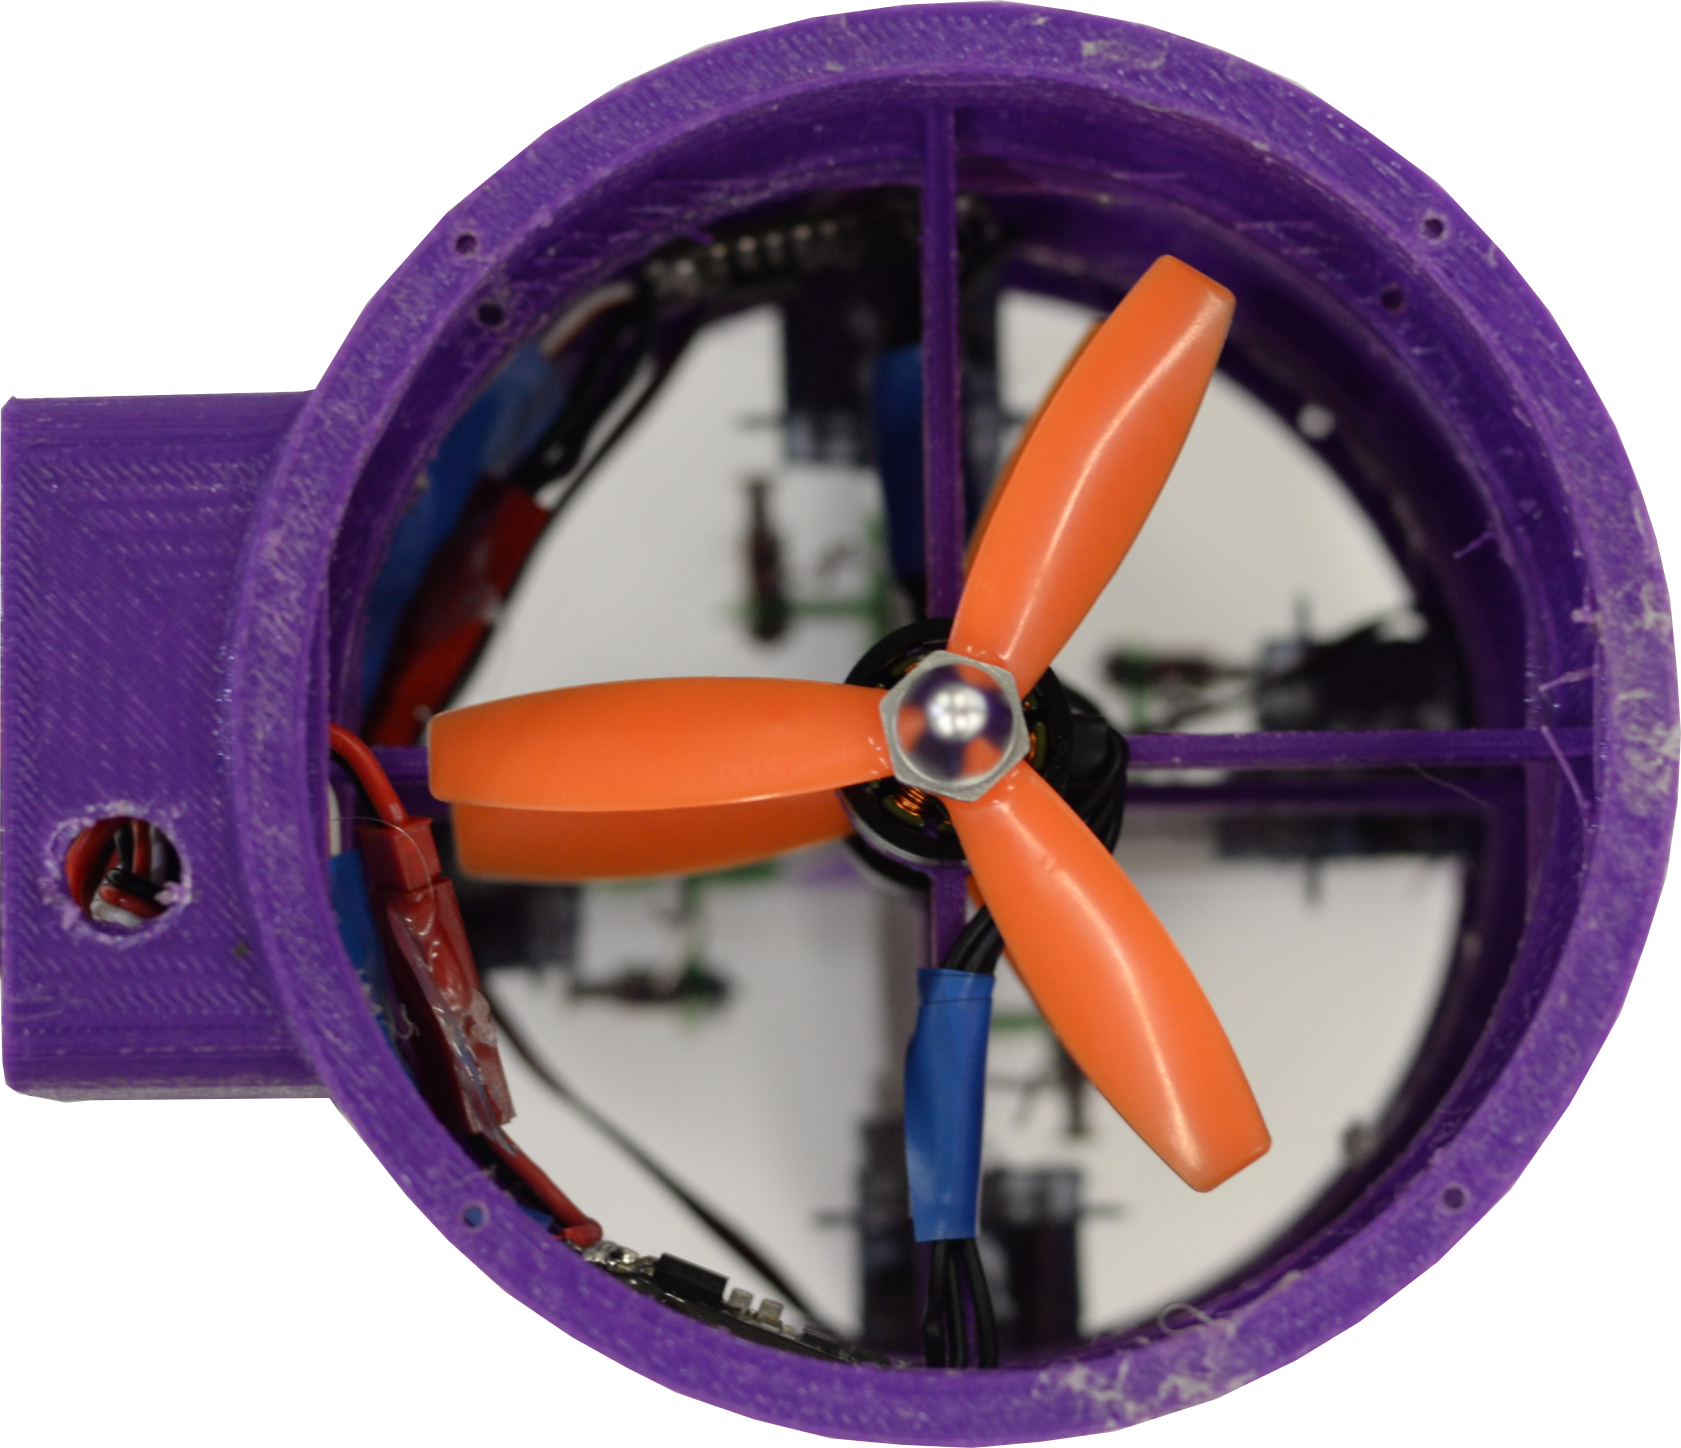
\includegraphics[width=0.9\linewidth]{sb-topdown.png}
		\caption{Top-down view of the SentiBot}
		\label{fig:sb-topdown}
	\end{subfigure}%
	\begin{subfigure}{0.5\textwidth}
		\centering
		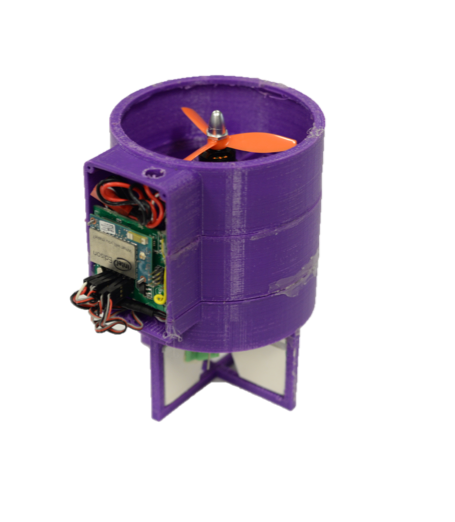
\includegraphics[width=0.9\linewidth]{sb-side.png}
	\caption{Perspective view of the SentiBot}
	\label{fig:sb-side}
	\end{subfigure}
\end{figure}

\subsection{Control system and steering}

Control and steering is accomplished through 4 thrust vectoring vanes manipulated by 3.3g 5v servos. Such a configuration is typical of other coax-copters as well.[15] The vanes are housed within protective housing to minimize damage during a collision. The servos are housed inside the frame with access panel doors to enabling replacement of damaged components. The frame encloses all moving components and aids in increasing the safety of using the platform.

\subsection{Motor-Propeller combination}

By spinning counter-rotating bullnose propellers using a 4000kV race quad motor, the SentiBot can achieve a high thrust to space ratio. Performance analysis of propellers show that larger diameter propellers are more efficient as compared to smaller propellers.[18] The SentiBot uses 2 large rotors arranged in a stacked configuration as compared to a quadrotor which uses 4 smaller propellers arranged in a plane thus higher efficiency can be obtained from the SentiBot.[18] This allows for a compact frame design while preserving the payload carrying capacity.

\subsection{Usage of a coaxial dual-motor thrust design}

\begin{table}[b]
	\centering
	\begin{tabular}{ | l | l l | }
		Configuration & Maximum Thrust/g & Maximum Current/A \\
		\hline
		A & 200 & 18 \\
		B & 250 & 13 \\
		C & 450 & 23 \\
	\end{tabular}
	\caption{Hardware components of the SentiBot}
	\label{fig:sb-configs}
\end{table}

Experiments were conducted to determine the motor configuration that would be the most ideal. 3 unique configurations where chosen for testing. Configuration A uses a single 4000kv Electronic Ducted Fan (EDF).  Configuration B utilizes a single 4000kv Racing Quadcopter motor which is spinning a 3040 triple blade propeller. Configuration C uses 2 4000kv motors spinning the same 3040 triple blade propeller stacked vertically with an inter-propeller distance of 8cm. Configuration C is significant as it accounts for the counter-torque effects produced by the motor and offers a method to cancel the effects unlike the preceding configurations which require active compensation from the control surfaces.

Each of these configurations, were tested by measuring the thrust output and current consumption and taking the average of 10 measurements. These results allow computation of the efficiency and maximum thrust output provided by each configuration. Given the battery capacity, flight time expectations and the mass of the SentiBot, the ideal configuration for the SentiBot can be determined.

\subsection{Jointed control surfaces}

4 servos were utilized to manipulate 4 independently movable control surfaces. Each servo weighs 3.3g and the duplicated, redundant control surfaces adds to the weight of drone. The removal of 2 of the servos, requires the control coupling of the 2 adjacent control surfaces which could lead to the loss of the additional yaw authority provided by independent control surfaces. The double motor configuration allows for enough yaw authority, so the adjacent control surfaces were coupled together using a jointed control surface design.

\subsection{Motor mounting struts}

The motor mounting struts where initially flattened on the positive Z-axis which resulted in the impedance of air flow resulting in loss of motor efficiency. Thus, the design was improved such that the motor-mounting strut is flattened on the positive X-axis which gives the strength and rigidity required of a motor mount while preventing air-flow impedance through the frame.

\subsection{Aerodynamic analysis of the frame}

The frame underwent aerodynamic analysis to determine the efficiency and drag co-efficient of the frame. Through this analysis, the frame can be ensured to be streamlined and to allow for efficient movement during operation. It additionally allows for a higher speed during flight.

\begin{figure}[t]
	\centering
	\begin{subfigure}{0.5\textwidth}
		\centering
		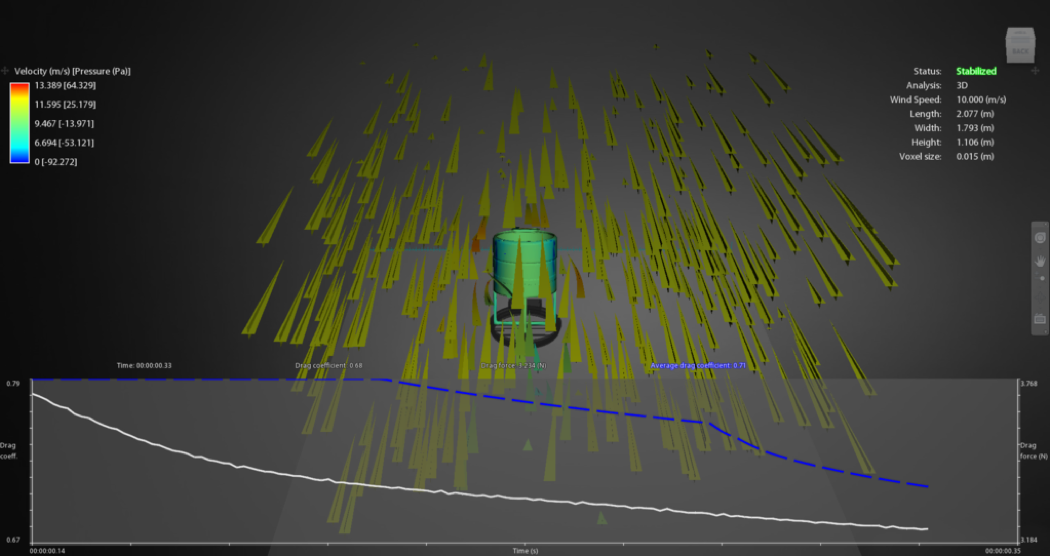
\includegraphics[width=0.9\linewidth]{aerodynamic-1.png}
	\end{subfigure}%
	\begin{subfigure}{0.5\textwidth}
		\centering
		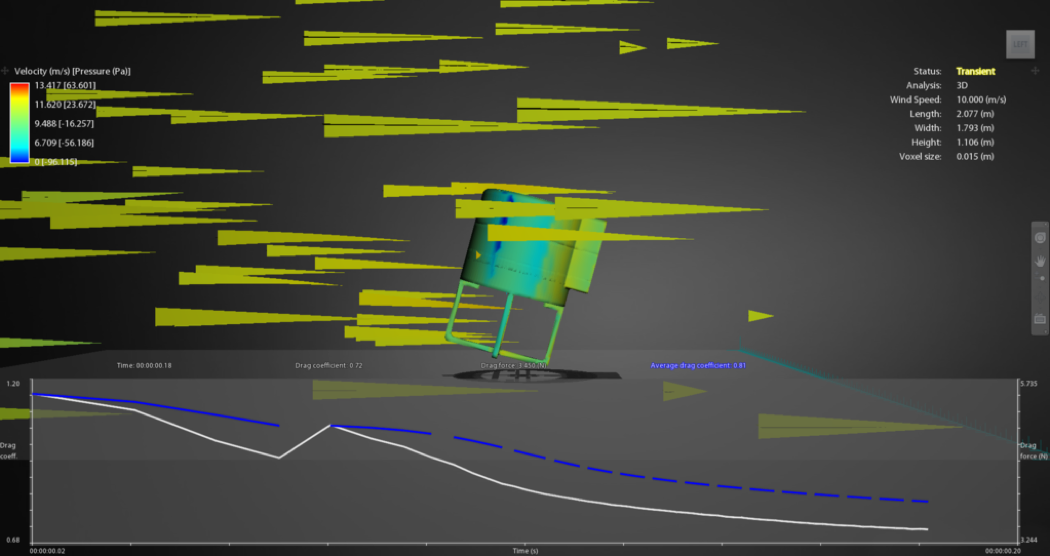
\includegraphics[width=0.9\linewidth]{aerodynamic-2.png}
	\end{subfigure}
	\caption{Meow}
	\label{fig:aerodynamic}
\end{figure}

The aerodynamic analysis of the frame in figure \ref{fig:aerodynamic} shows that due to the cylindrical frame design, the body is minimized. During forward motion, the drag primarily arises from the electronics compartment but it is considered negligible as the craft is too small for these effects to manifest in a significant manner. The one-sided nature of the electronics compartment results in the loss of radial symmetry which gives rise to some instability but the software mechanisms have been designed and tuned to compensate for these errors.

\begin{table}[h]
	\centering
	\begin{tabular}{ | l | l | }
		Component & Hardware \\
		\hline
		Main Processor & Dual core 500Mhz Intel Atom \\
		Secondary Processor & ATMEGA 328 \\
		Motors & 4000KV motors \\
		ESCs & 12A XMS series \\
		Batteries & 800mAh 4S(14.8v) \\
		Propellers & 3x3x4.5 \\
		Servos & 2.8g ultralight \\
		Thrust & 500g \\
		Weight & 250g \\
	\end{tabular}
	\caption{Hardware components of the SentiBot}
	\label{fig:sb-components}
\end{table}

\section{SentiBot Electronics Design}

\subsection{Main Processor}

A powerful onboard processor as computing power intensive tasks cannot be offloaded to a ground-station when research like swarm intelligence and decentralized computing[19] is being conducted. Vision processing and autonomous navigation also are very computing intensive[21]. The SentiBot has an Intel Edison SoC which consists of a 500Mhz Intel Atom, an Intel Quark microcontroller, 1GB of onboard DDR3 RAM and 4GB of onboard flash storage.[22] 

\subsection{Dual CPU architecture}

An ATmega 328 microcontroller is used as a secondary processor to provide more General Purpose IO (GPIO) and sensor extensibility. A dual-layer PCB was designed to integrate the Intel Edison and the ATmega in a dual-CPU architecture. Higher-level tasks are executed in the Intel Edison while time-critical tasks like communication with sensors and actuators are done in the ATmega 328. The separation of the higher and lower level processing also provides code organization in the software.

\subsection{On board sensors}

The main sensor which allows for the drone to fly in a stable manner is the Inertial Measurement Unit (IMU). This sensor provides accelerometer and gyroscope information to the ATmega 328 for the PID loop to keep the drone upright. The sensor also allows for dead reckoning to be used for localization.[23]

The IR distance sensors mounted on all 4 sides allows for collision avoidance to prevent crashes. There is also an onboard RGB camera which interfaces to the primary processor over USB. 

\subsection{Flight Drive system specifications}

The power electronics consists of 4 1C 1200mAh batteries, 2 30A super light Electronic Speed Controllers (ESC) and 2 4000kV 1306 motors. The motors have a max current draw of 8A each and taking into consideration that the max thrust of each motor is 370g the gram per current rating for each motor is 46g/A. Since the weight of the SentiBot is about 320g, the nominal current draw during a hover would be about 7A. That gives a flight time of about 10-15 minutes. 

\subsection{Power Supply management}

In terms of power management, 3 voltage levels are required - 14.8V from the battery, 5V for the control board and 3.3V for the control circuity. Since the drone’s ESCs do not come equipped with a built in battery eliminator circuit (BEC) an external switching regulator is used to supply clean 5V for the control board. The onboard 3.3V LDO further steps down the voltage from 5V to 3.3V

\section{Software Design}

SentiBots has two methods of operation: manual and autonomous. In manual, an operator has full control and information from the drone. Operated autonomously, the drone is user-programed to complete tasks with little or no human intervention. SentiBots has two subsystems: control and intelligence. The control subsystem consists of the hardware interface to GPIO and the Inertial Measurement Unit (IMU), and relevant Proprotional Integral Derevative (PID) loops. It also can provide basic obstacle avoidance. The intelligence subsystem is for complex tasks like navigation, localization, vision, object identification and other tasks for autonomous flight. It also provides communication with the groundstation.

\subsection{Lower level subsystem}

The control algorithm in SentiBot is standard. Sensor data is mapped into error values that can be used to compensate for frame errors and instabilities. IMU data (processed by an internal Digital Signal Processor) is read over I^2C to obtain yaw-pitch-roll (YPR) data. Each YPR value is used in PID loops for each axis to obtain error values. The angle of the control surfaces are set by the error values, therefore stabilizing the system. This computation runs on the ATmega 328.

As shown in figure \ref{fig:intelsystem}, A I^2C peripheral interface is used between the lower level subsystem and the IMU. A USART interface is used between the microcontroller and the processor running the higher level subsystem. This communication is managed by software that utilizes the Multi-Wii protocol.[5]

The firmware which runs the lower level subsystem is based on the open-source Multi-Wii project. Minor modifications were made to the firmware for coax-copter support but the built-in Multi-Wii PID loop controller and communication infrastructure were used. The open-source Multi-Wii framework is modular and easy to modify for the end user. The Multi-Wii platform is also well documented and easy to understand. The lower level subsystem carries out basic collision avoidance system with 4 IR sensors installed around the bot. This prevents higher level algorithms from allowing crashes and damage to the bot and the environment. This is done through a modification that is made to the Multi-Wii framework which adds collision avoidance functionality to it.

\subsection{Higher Level subsystem}

The autonomy of the SentiBots, when implemented in a fully modular manner, allows students to tap onto resources available online and libraries for implementing autonomy in the SentiBots. Thus, the SentiBots is based on the ROS architecture which is completely open source and provides existing libraries for students to easily implement systems into the robots. The ROS architecture is already used by students and researchers.

The communication system is reliant on the onboard WiFi chipset present in the Intel Edison SoC. It connects to an 802.11n network operated by the ground station and transmits over the established network. It also transmits telemetry information gathered from hardware through the microcontroller and sensor expansion port.

\subsection{Ground-station software}

We are currently still in the process of designing and implementing the ground-station. However, we have developed a method to control it through an android app. It uses a simple UDP interface and connects to the Edison via WiFi which allows instructions to be issued to the SentiBot. Lately, a Spektrum satellite receiver has also been added to the spare UART2 port for longer range and lower latency. 

\section{Results}

The results of initial testing were positive. The SentiBot shows the ability to lift off, and fly in a stable hover with minimal user intervention. When moved around, the SentiBot platform can accurately maintain its attitude without much user compensation. Furthermore, the drop tests were significantly positive showing that the SentiBot can survive drops from up to 3m high due to its rigid 3D printed PLA frame. These drop tests were conducted through flying to robot up to a certain height and removing power from the motors and measuring how high we could drop from before there was damage to the frame. Only one test run was conducted. In testing, the top speed achieved from the SentiBot is also about 20km/h and flight times are about 15 minutes with normal flying. Furthermore, the SentiBot is able to achieve versatile flight through, under and over several obstacles without any problems due to its small size and form factor. The SentiBot can also easily take collisions with walls or other obstacles without falling due to its shell. 

\section{Conclusion}

The SentiBot project set out to bring an extremely safe, easy to use and cheap drone for use in educational institutions around the world. It aimed to solve some critical issues in bringing consumer drones to educational institutions for use in student interaction and learning processes by making an ideal drone platform that caters to the cost, ease of use and safety issues presented in those consumer drones. We have created that platform in SentiBots. The competitive pricing with consumer drones while providing one the safest and most hackable drones in the world today makes it highly suitable for educational institutions ranging from secondary schools to tertiary institutions and universities. 
Some future work could be conducted into more detailed software which can complement the SentiBot hardware platform as software support for coax-copters in the world today is very limited and rudimentary.

\section{References}

\bibliographystyle{plain}
\bibliography{report}

\end{document}
